\documentclass[11pt]{article}
\usepackage[margin=1in]{geometry}
\usepackage{amsmath, amssymb}
\usepackage{enumitem}
\usepackage{setspace}
\usepackage{tikz}
\usetikzlibrary{decorations.pathreplacing}
\usepackage{booktabs}

\setstretch{1.15}
\setlist[itemize]{leftmargin=1.5em}
\setlist[enumerate]{leftmargin=1.7em}

\setcounter{tocdepth}{2}

\begin{document}
\tableofcontents
\clearpage

\begin{center}
  {\Large Intermediate Macroeconomics --- Typed Notes}\\
  {\small (Transcription of the 60-page handwritten packet)}
\end{center}

\section*{CH.\ 2: Tour of the Book}

\subsection*{2-1 Aggregate Output}
\subsubsection*{GDP: Production \& Income}
\begin{enumerate}
  \item Value of final goods \& services produced domestically.
  \item Sum of value added by every producer in the economy.
  \item Sum of incomes earned in the economy.
\end{enumerate}

\subsubsection*{Nominal vs.\ Real GDP}
\[
  \text{Nominal GDP} = \sum (\text{quantity of final goods}) \times (\text{current prices}).
\]
Real GDP prices the same basket at constant prices to isolate the quantity effect.

\subsubsection*{GDP: Level vs.\ Growth}
\begin{enumerate}
  \item Output per capita $\rightarrow$ average standard of living.
  \item GDP growth:
  \[
    g_Y(t) = \frac{\Delta Y_t}{Y_{t-1}}
  \]
  \begin{itemize}
    \item Expansion: $\Delta Y_t > 0 \Leftrightarrow g_Y(t) > 0$.
    \item Recession: $\Delta Y_t < 0 \Leftrightarrow g_Y(t) < 0$.
  \end{itemize}
\end{enumerate}

\subsection*{2-2 Unemployment Rate}
\[
  L = N + U, \qquad u = \frac{U}{L} = 1 - \frac{N}{L}.
\]
Unemployment directly affects welfare; $u$ signals whether resources are efficiently allocated.

\begin{figure}[h]
  \centering
  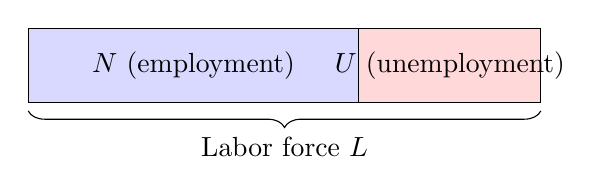
\begin{tikzpicture}[scale=1.05]
    \draw[fill=blue!15] (0,0) rectangle (4,0.9);
    \draw[fill=red!15] (4,0) rectangle (6.2,0.9);
    \draw (0,0) rectangle (6.2,0.9);
    \node at (2,0.45) {$N$ (employment)};
    \node at (5.1,0.45) {$U$ (unemployment)};
    \draw[decorate,decoration={brace,amplitude=6pt,mirror}] (0,-0.1) -- (6.2,-0.1)
      node[midway,below=6pt]{Labor force $L$};
  \end{tikzpicture}
  \caption{Labor-force composition.}
\end{figure}

\subsection*{2-3 Inflation Rate}
\[
  P_t = \frac{\$Y_t}{Y_t^{\text{real}}}, \qquad \pi_t = \frac{\Delta P_t}{P_{t-1}}.
\]
\begin{itemize}
  \item GDP deflator $= \dfrac{\text{nominal GDP}_t}{\text{real GDP}_t} \Longleftrightarrow P_t$.
  \item Inflation $\pi_t = \dfrac{\Delta P_t}{P_{t-1}} = g(P_t)$.
  \item CPI = cost in dollars of a fixed basket of goods and services.
  \item GDP deflator tends to move with the CPI.
\end{itemize}

\subsection*{2-4 Okun's Law \& Phillips Curve}
\begin{description}
  \item[Okun's Law:] Negative relation between GDP growth $g_Y(t)$ and the change in unemployment $\Delta u_t$.
  \item[Phillips Curve:] Negative relation between the change in inflation $\Delta \pi_t$ and unemployment $u_t$.
\end{description}

\begin{figure}[h]
  \centering
  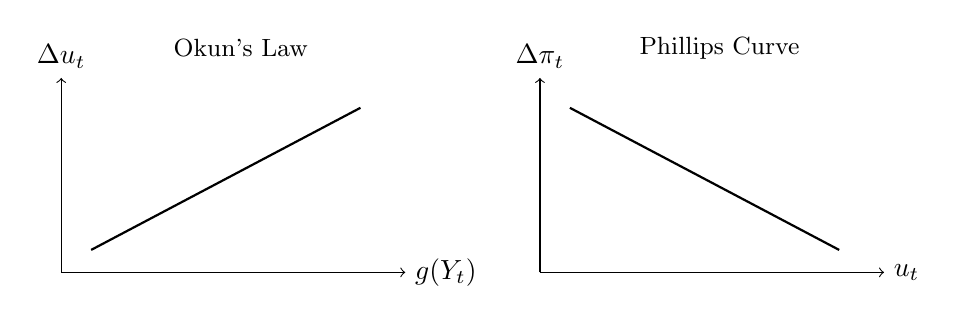
\begin{tikzpicture}[scale=0.95]
    \begin{scope}
      \node at (2.4,3) {\small Okun's Law};
      \draw[->] (0,0) -- (4.6,0) node[right] {$g(Y_t)$};
      \draw[->] (0,0) -- (0,2.6) node[above] {$\Delta u_t$};
      \draw[thick] (0.4,0.3) -- (4,2.2);
    \end{scope}
    \begin{scope}[xshift=6.4cm]
      \node at (2.4,3) {\small Phillips Curve};
      \draw[->] (0,0) -- (4.6,0) node[right] {$u_t$};
      \draw[->] (0,0) -- (0,2.6) node[above] {$\Delta \pi_t$};
      \draw[thick] (0.4,2.2) -- (4,0.3);
    \end{scope}
  \end{tikzpicture}
  \caption{Axes mirrored exactly as in the handwritten Okun's Law and Phillips Curve sketches.}
\end{figure}

\section*{CH.\ 3: The Goods Market}

\subsection*{3-1 Composition of GDP}
\[
  Y = C + I + G + NX.
\]
\begin{itemize}
  \item Government purchases $G$ exclude transfers (Medicare, Social Security, interest on debt). Transfers $\approx 39\%$ of total outlays.
  \item US GDP 2010 shares: $C \approx 70.5\%$, $I \approx 12\%$, $G \approx 20.4\%$, $NX \approx -3\%$.
  \item Production $Y$ equals sales $(C+I+G+NX)$ plus inventory investment ($\approx 0.5\%$ in 2010).
\end{itemize}

\subsection*{3-2 Demand for Goods}
Demand:
\[
  Z = C + I + G + X - IM.
\]
Assumptions:
\begin{enumerate}
  \item Single composite good produced by all firms.
  \item Firms supply any $Q$ at the given $P$.
  \item Closed economy baseline $\Rightarrow X = IM = 0$.
\end{enumerate}
Disposable income $Y_D = Y - T$. Consumption $C = c_0 + c_1 Y_D$ with $c_0 > 0$ and $c_1 = \text{MPC}$. Investment $\bar{I}$ and $(\bar{G},\bar{T})$ exogenous.

\subsection*{3-3 Determination of Equilibrium Output}
\[
  Y = c_0 + c_1 (Y - T) + \bar{I} + G
  \quad \Rightarrow \quad
  Y = \frac{1}{1 - c_1}\left(c_0 + \bar{I} + G - c_1 T\right).
\]
The multiplier on autonomous spending is $\frac{1}{1-c_1}$. With $G=T$ the autonomous component is positive. US MPC $\approx 0.6$ so multipliers are moderate.

\begin{figure}[h]
  \centering
  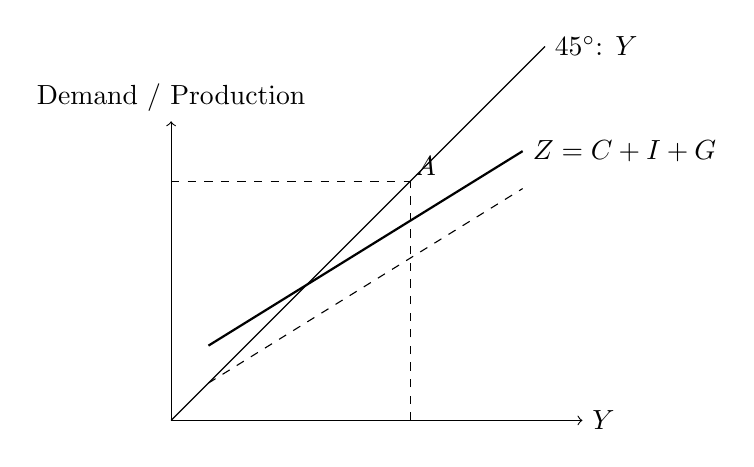
\begin{tikzpicture}[scale=0.95]
    \draw[->] (0,0) -- (5.5,0) node[right] {$Y$};
    \draw[->] (0,0) -- (0,4) node[above] {Demand / Production};
    \draw (0,0) -- (5,5) node[right] {$45^\circ$: $Y$};
    \draw[thick] (0.5,1) -- (4.7,3.6) node[right] {$Z = C+I+G$};
    \draw[dashed] (0.5,0.5) -- (4.7,3.1);
    \draw[dashed] (3.2,0) -- (3.2,3.2);
    \draw[dashed] (0,3.2) -- (3.2,3.2);
    \node at (3.4,3.4) {$A$};
  \end{tikzpicture}
  \caption{Keynesian cross: equilibrium where $Z=Y$.}
\end{figure}

\subsection*{3-4 Investment Equals Saving}
\begin{align*}
  S_{\text{private}} &= Y - T - C,\\
  S_{\text{public}} &= T - G,\\
  I &= S_{\text{private}} + S_{\text{public}}.
\end{align*}
Private saving schedule: $S = -c_0 + (1 - c_1)(Y - T)$ with $1 - c_1 = \text{MPS}$. Budget surplus ($T>G$) vs.\ deficit ($T<G$).

\section*{CH.\ 4: Financial Markets}

\subsection*{4-1 Demand for Money}
\begin{itemize}
  \item Money = currency (coins/bills) + checkable deposits. $M1 =$ currency $+$ checkable deposits.
  \item Bonds pay interest $i$ but cannot execute transactions.
  \item Portfolio choice depends on transaction needs and $i$ (opportunity cost of holding money).
  \item Money demand: $M^d = \$Y \cdot f(i)$ with $f' < 0$.
\end{itemize}

\begin{figure}[h]
  \centering
  \begin{tikzpicture}[scale=1]
    \draw[->] (0,0) -- (0,3.2) node[above] {$i$};
    \draw[->] (0,0) -- (4.8,0) node[right] {$M$};
    \draw[thick] (0.5,2.8) -- (4.2,0.5) node[right] {$M^d$};
    \draw[thick] (2.8,0) -- (2.8,2.9) node[above] {$M^s$};
  \end{tikzpicture}
  \caption{Money demand and vertical money supply exactly as sketched in the notes.}
\end{figure}

\subsection*{4-2 Determining the Interest Rate}
Equilibrium satisfies $M^s = M^d$.
\begin{itemize}
  \item $\uparrow M^s \Rightarrow \downarrow i$ (for fixed $\$Y$).
  \item $\uparrow \$Y \Rightarrow \uparrow i$ (for fixed $M^s$).
\end{itemize}

\subsection*{4-3 Monetary Policy \& Open-Market Operations}
\begin{enumerate}
  \item Expansionary: buy bonds $\Rightarrow \uparrow M^s$.
  \item Contractionary: sell bonds $\Rightarrow \downarrow M^s$.
\end{enumerate}
One-year T-bill price $P_B = \dfrac{c}{1 + i}$ (inverse relation between $i$ and bond price). Fed targets an interest rate $i^\ast$ via money supply.

\subsection*{4-3b Determining Interest Rate (II)}
Balance sheets:
\begin{itemize}
  \item Central bank: assets = bonds, liabilities = reserves $+$ currency (central bank money).
  \item Banks: assets = reserves/loans/bonds, liabilities = checkable deposits; must satisfy reserve ratio.
\end{itemize}

\subsection*{4-4 Demand for Central Bank Money}
\begin{align*}
  C^d &= c M^d, \quad D^d = (1-c)M^d, \quad R^d = \theta D^d,\\
  H^d &= C^d + R^d = [c + \theta (1-c)]\,\$Y \cdot f(i).
\end{align*}
Money multiplier $= \dfrac{1}{c + \theta(1-c)}$. Fed funds rate determined by reserve market. Overall money supply-demand condition:
\[
  \frac{1}{c+\theta(1-c)}\,H = \$Y \cdot f(i).
\]

\begin{figure}[h]
  \centering
  \begin{tikzpicture}[scale=1]
    \draw[->] (0,0) -- (0,3.2) node[above] {$i$};
    \draw[->] (0,0) -- (4.8,0) node[right] {$H$};
    \draw[thick] (0.5,2.7) -- (4.2,0.6) node[right] {$H^d$};
    \draw[thick] (2.6,0) -- (2.6,2.9) node[above] {$H^s$};
    \node at (1.1,2.85) {$A$};
  \end{tikzpicture}
  \caption{Market for central bank money (reserves) mirroring the handwritten diagram.}
\end{figure}

\section*{CH.\ 5: Goods \& Financial Markets --- IS/LM}

\subsection*{5-1 Goods Market \& IS Relation}
Equilibrium:
\[
  Y = C(Y-T) + I(Y,i) + G.
\]
Higher $i$ lowers demand both directly (via $I$) and indirectly (via $Y$), giving a downward-sloping IS.

\begin{figure}[h]
  \centering
  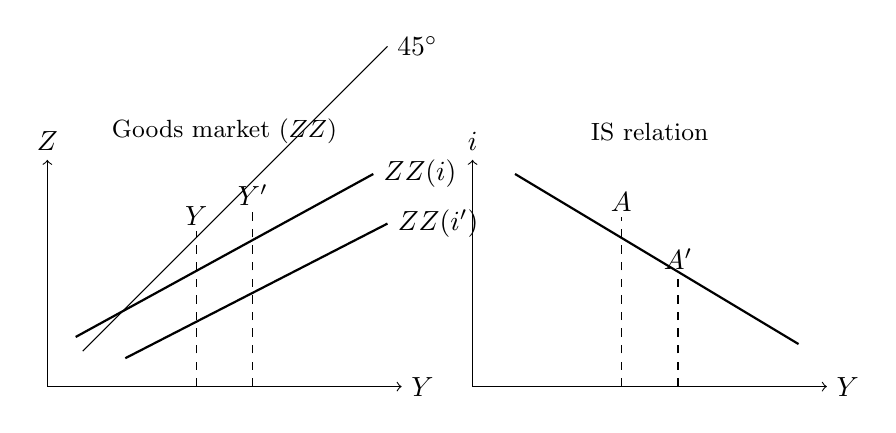
\begin{tikzpicture}[scale=0.9]
    \begin{scope}
      \node at (2.5,3.6) {\small Goods market ($ZZ$)};
      \draw[->] (0,0) -- (5,0) node[right] {$Y$};
      \draw[->] (0,0) -- (0,3.2) node[above] {$Z$};
      \draw (0.5,0.5) -- (4.8,4.8) node[right] {$45^\circ$};
      \draw[thick] (0.4,0.7) -- (4.6,3.0) node[right] {$ZZ(i)$};
      \draw[thick] (1.1,0.4) -- (4.8,2.3) node[right] {$ZZ(i')$};
      \draw[dashed] (2.1,0) -- (2.1,2.2);
      \draw[dashed] (2.9,0) -- (2.9,2.5);
      \node at (2.1,2.4) {$Y$};
      \node at (2.9,2.7) {$Y'$};
    \end{scope}
    \begin{scope}[xshift=6cm]
      \node at (2.5,3.6) {\small IS relation};
      \draw[->] (0,0) -- (5,0) node[right] {$Y$};
      \draw[->] (0,0) -- (0,3.2) node[above] {$i$};
      \draw[thick] (0.6,3.0) -- (4.6,0.6);
      \draw[dashed] (2.1,0) -- (2.1,2.4);
      \draw[dashed] (2.9,0) -- (2.9,1.6);
      \node at (2.1,2.6) {$A$};
      \node at (2.9,1.8) {$A'$};
    \end{scope}
  \end{tikzpicture}
  \caption{Goods-market diagram and associated IS schedule as drawn in the handwritten notes.}
\end{figure}

\subsection*{5-2 Financial Markets \& LM Relation}
Money-market equilibrium:
\[
  \frac{M}{P} = Y \cdot f(i).
\]
Higher $Y$ shifts money demand up $\Rightarrow$ higher $i$ for a given $M/P$. Higher money supply shifts LM down.

\subsection*{5-3 Putting IS \& LM Together}
Intersection of IS and LM pins down $(Y,i)$. Short run assumes fixed $P$ (empirically reasonable) so there is a single relevant interest rate (short- and long-term move together).

\begin{figure}[h]
  \centering
  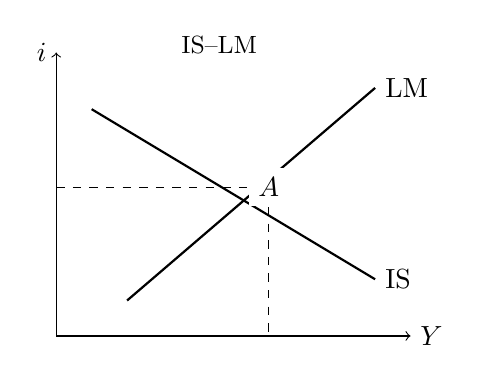
\begin{tikzpicture}[scale=0.9]
    \begin{scope}
      \node at (2.3,4.1) {\small IS--LM};
      \draw[->] (0,0) -- (0,4) node[left] {$i$};
      \draw[->] (0,0) -- (5,0) node[right] {$Y$};
      \draw[thick] (0.5,3.2) -- (4.5,0.8) node[right] {IS};
      \draw[thick] (1,0.5) -- (4.5,3.5) node[right] {LM};
      \draw[dashed] (0,2.1) -- (3,2.1) -- (3,0);
      \node[fill=white] at (3,2.1) {$A$};
    \end{scope}
  \end{tikzpicture}
  \caption{IS--LM equilibrium.}
\end{figure}

\subsection*{Policy Effects}
\begin{itemize}
  \item Fiscal contraction (lower $G-T$): IS $\leftarrow$, $Y \downarrow$, $i \downarrow$, movement along LM.
  \item Fiscal expansion: IS $\rightarrow$, $Y \uparrow$, $i \uparrow$.
  \item Monetary expansion ($\uparrow M$): LM $\downarrow$, $Y \uparrow$, $i \downarrow$.
\end{itemize}

\subsection*{Summary Box}
\begin{center}
\begin{tabular}{@{}lcccc@{}}
\toprule
Policy & IS shift & LM shift & $\Delta Y$ & $\Delta i$ \\
\midrule
$\uparrow$ Taxes & $\leftarrow$ & None & $\downarrow$ & $\downarrow$ \\
$\downarrow$ Taxes & $\rightarrow$ & None & $\uparrow$ & $\uparrow$ \\
$\uparrow$ Spending & $\rightarrow$ & None & $\uparrow$ & $\uparrow$ \\
$\downarrow$ Spending & $\leftarrow$ & None & $\downarrow$ & $\downarrow$ \\
$\uparrow$ Money & None & $\downarrow$ & $\uparrow$ & $\downarrow$ \\
$\downarrow$ Money & None & $\uparrow$ & $\downarrow$ & $\uparrow$ \\
\bottomrule
\end{tabular}
\end{center}

\subsection*{Fiscal \& Monetary Policy Examples}
\begin{itemize}
  \item \textbf{Fiscal contraction (consolidation):} $\downarrow(G-T)$ via $\downarrow G$ or $\uparrow T$.
  \[
    \downarrow G \Rightarrow \downarrow Y_d \Rightarrow \downarrow C \Rightarrow \downarrow Y \Rightarrow \downarrow M^d.
  \]
  With $i$ fixed, the economy moves along LM from $Y_1$ to $Y_2$.
  \item \textbf{Fiscal expansion:} $\uparrow(G-T)$ shifts IS right, raising $Y$, $i$, $C$, and---for a given $i$---induces further $\uparrow Y$ to restore LM equilibrium.
  \item \textbf{Monetary expansion:} $\uparrow M^s \Rightarrow \downarrow i$, boosting $I$ and shifting IS right; outcome $\uparrow Y$, $\uparrow C$, $\uparrow I$, $\uparrow E$ (depreciation), $NX$ ambiguous.
  \item \textbf{Monetary contraction:} $\downarrow M^s \Rightarrow \uparrow i$, reducing $I$, $Y$, $C$, appreciating the currency, and lowering $NX$.
\end{itemize}

\subsection*{Liquidity Trap Supplement}
\begin{itemize}
  \item When $i$ hits its lower bound, LM becomes horizontal: $\uparrow M$ no longer lowers $i$.
  \item Credit or quantitative easing can shift LM modestly but mainly fiscal policy is effective.
  \item In AD--AS space the AD curve becomes vertical because $M/P$ changes cannot move $i$.
\end{itemize}

\section*{CH.\ 6: The Labor Market}

\subsection*{6-1 Tour of Labor Market (US 2010)}
\begin{itemize}
  \item Total population: 308.7M; non-institutional civilian pop: 237.8M.
  \item Labor force: 153.8M $\Rightarrow$ participation rate $\approx 64.7\%$.
  \item Employment $E=139$M, unemployment $U=14.8$M $\Rightarrow u \approx 9.6\%$.
  \item Flows arise continuously via separations and hires.
\end{itemize}

\subsection*{6-2 Movements in Unemployment}
\begin{itemize}
  \item Annual changes in aggregate $u$ align with recessions/expansions.
  \item If $u$ is high:
    \begin{enumerate}
      \item Probability of job loss for employed workers rises.
      \item Probability of job finding for unemployed falls.
    \end{enumerate}
\end{itemize}

\subsection*{6-3 Wage Determination}
\begin{itemize}
  \item Collective bargaining between unions and firms.
  \item Reservation wage makes workers indifferent between working and being unemployed.
  \item Wage $>$ reservation wage reduces turnover.
  \item Bargaining power rises with higher replacement cost for firms and limited alternative jobs for workers.
\end{itemize}

\subsection*{Efficiency Wages \& Price Setting (6-4)}
\[
  W = P^e F(u,z),
\]
where $z$ captures unemployment insurance, employment protection, etc. Price-setting: $P = (1 + m)W$.

\subsection*{6-5 Natural Rate of Unemployment}
Assuming $P^e = P$ in the medium run:
\[
  F(u_n, z) = \frac{1}{1 + m}.
\]
Higher unemployment benefits (higher $z$) or higher markup $m$ raise $u_n$ by shifting WS or lowering PS.

\subsection*{Natural Employment \& Output}
\[
  N_n = L(1 - u_n), \qquad Y_n = A N_n.
\]
In the normalized notes $A=1$, so $Y_n = N_n$. WS-PS differs from standard labor supply/demand:
\begin{enumerate}
  \item Wage determined through bargaining vs.\ worker willingness to work.
  \item Firms set prices/wages vs.\ price-taking in competitive model.
  \item Involuntary unemployment present at equilibrium.
\end{enumerate}

\section*{CH.\ 7: The AS--AD Model}

\subsection*{7-1 Aggregate Supply}
\begin{align*}
  W &= P^e F(u,z),\\
  P &= (1+m)W, \\
  u &= 1 - \frac{Y}{L}.
\end{align*}
Thus $P = P^e (1+m) F\!\left(1 - \frac{Y}{L}, z\right)$. Properties:
\begin{enumerate}
  \item Given $P^e$, $\uparrow Y \Rightarrow \downarrow u \Rightarrow \uparrow W \Rightarrow \uparrow P$.
  \item Given $u$, $\uparrow P^e \Rightarrow \uparrow P$ one-for-one.
  \item $Y = Y_n \Rightarrow u = u_n \Rightarrow P = P^e$.
\end{enumerate}

\subsection*{7-2 Aggregate Demand}
Derived from IS--LM:
\[
  Y = Y\!\left(\frac{M}{P}, G, T\right).
\]
Given $(M,G,T)$, higher $P$ lowers $M/P$ and shifts LM up, so AD slopes downward. Any factor shifting IS or LM shifts AD.

\subsection*{7-3 Short-Run vs.\ Medium-Run Equilibrium}
\begin{itemize}
  \item Short run: intersection of AS and AD determines $(Y,P)$ with $P^e$ given.
  \item Medium run: $P^e$ adjusts so that $Y \rightarrow Y_n$.
\end{itemize}

\begin{figure}[h]
  \centering
  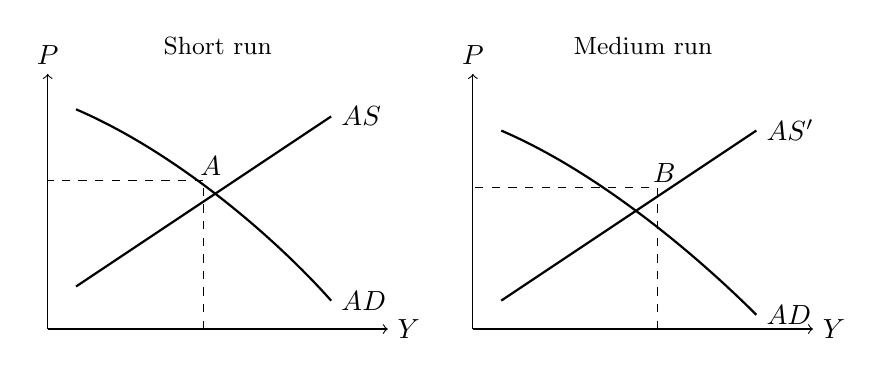
\begin{tikzpicture}[scale=0.9]
    \begin{scope}
      \node at (2.4,4) {\small Short run};
      \draw[->] (0,0) -- (4.8,0) node[right] {$Y$};
      \draw[->] (0,0) -- (0,3.6) node[above] {$P$};
      \draw[thick] (0.4,0.6) -- (4,3) node[right] {$AS$};
      \draw[thick] (0.4,3.1) .. controls (1.8,2.5) and (3.2,1.3) .. (4.0,0.4) node[right] {$AD$};
      \draw[dashed] (2.2,0) -- (2.2,2.1) -- (0,2.1);
      \node at (2.3,2.3) {$A$};
    \end{scope}
    \begin{scope}[xshift=6.0cm]
      \node at (2.4,4) {\small Medium run};
      \draw[->] (0,0) -- (4.8,0) node[right] {$Y$};
      \draw[->] (0,0) -- (0,3.6) node[above] {$P$};
      \draw[thick] (0.4,0.4) -- (4,2.8) node[right] {$AS'$};
      \draw[thick] (0.4,2.8) .. controls (1.8,2.2) and (3.2,1.0) .. (4.0,0.2) node[right] {$AD$};
      \draw[dashed] (2.6,0) -- (2.6,2.0) -- (0,2.0);
      \node at (2.7,2.2) {$B$};
    \end{scope}
  \end{tikzpicture}
  \caption{AS--AD diagrams showing the short-run and medium-run movements back to $Y_n$.}
\end{figure}

\subsection*{7-4 Effects of Monetary Expansion}
\begin{itemize}
  \item $\uparrow M$ shifts AD right $\Rightarrow Y\uparrow$, $P\uparrow$, $i\downarrow$ in the short run.
  \item Over time, lower unemployment raises wages and shifts AS up; $Y$ returns to $Y_n$ while $P$ stays higher (neutrality of money in the medium run).
\end{itemize}

\subsection*{7-5 Decrease in Budget Deficit}
\begin{itemize}
  \item $\downarrow G$ (with constant $M$) shifts AD left $\Rightarrow \downarrow Y$, $\downarrow P$, $\downarrow i$ in short run.
  \item Falling $P$ raises real money supply, shifting LM down; AS eventually adjusts so $Y$ returns to $Y_n$ with lower $P$ and $i$.
  \item Composition of demand changes: lower $G$, higher $I$ (crowding in).
\end{itemize}

\subsection*{7-6 Increase in Price of Oil}
\begin{itemize}
  \item Higher oil price raises production costs $\Rightarrow$ higher markup $m$ for given $W$.
  \item Lowers real wage, raises $u_n$, lowers $Y_n$.
  \item Short run: AS shifts left through point $B$; medium run: AS keeps shifting (if oil price permanent) to $AS''$; AD also shifts as expectations adapt.
  \item 2000s vs.\ 1970s: (1) workers had less bargaining power so accepted smaller real-wage cuts (smaller AS shift), (2) monetary policy was more credible so inflation expectations stayed anchored.
\end{itemize}

\section*{CH.\ 8: Phillips Curve, $u_n$, \& Inflation}

\subsection*{8-1 $\pi$, $\pi^e$, and Unemployment}
With $F(u,z) = 1 - \alpha u + z$:
\[
  \pi_t = \pi_t^e + (m + z) - \alpha u_t.
\]

\subsection*{8-2 Phillips Curve Evolution}
\begin{itemize}
  \item Early Solow--Samuelson: $\pi_t = (m+z) - \alpha u_t$ (assumes $\pi_t^e=0$).
  \item 1970s: expectations became adaptive, $\pi_t^e = \theta \pi_{t-1}$ with $\theta$ rising toward 1.
  \item Post-1970 estimate: $\pi_t - \pi_{t-1} = 3.3\% - 0.55 u_t$.
  \item Friedman/Phelps: stable trade-off requires wage-setters to systematically underpredict inflation.
\end{itemize}

\subsection*{8-3 Summary \& Warnings}
\begin{itemize}
  \item 1979 Volcker disinflation: tighten monetary policy, accept higher $u$ to reduce $\pi$.
  \item Lucas critique: policy changes alter expectations; credibility matters.
  \item Wage indexation model with share $\lambda$ indexed:
  \[
    \pi_t = \lambda \pi_t + (1-\lambda)\pi_{t+1}^e - \alpha (u_t - u_n).
  \]
  Higher $\lambda$ dampens the effect of $u_t - u_n$ on inflation.
  \item Deflation undermines Phillips relationship because indexation behaves differently when $\pi < 0$.
\end{itemize}

\subsection*{Neutrality of Money}
In steady state,
\[
  Y_n = Y\!\left(\frac{M}{P}, G, T\right)
  \quad \Rightarrow \quad
  \pi = g_M
\]
if fiscal policy is unchanged. Price-level changes that do not affect money growth have no long-run effect on inflation.

\section*{CH.\ 9: The Crisis}

\subsection*{9-1 From Housing Problem to Financial Crisis}
\begin{itemize}
  \item Housing prices (Case--Shiller) surged 2000--06 due to low mortgage rates and rapid growth of subprime lending; plunged 2006--09.
  \item Mortgages went underwater; many risky NINJA loans became toxic.
  \item Banks as intermediaries: Assets = Liabilities $+$ Capital. Insolvency $(A<L)$ vs.\ illiquidity (insufficient liquid assets).
  \item Leverage ratio $= \frac{A}{C}$: high leverage $\Rightarrow$ higher expected returns but higher insolvency risk.
  \item Complex securitization (MBS, CDO tranches) made valuation difficult; when underlying mortgages defaulted, securities became ``toxic.''
\end{itemize}

\subsection*{9-2 Use \& Limits of Policy}
\begin{itemize}
  \item Liquidity/wholesale funding: banks borrowed short-term to finance long-term assets; fire sales depressed prices.
  \item TED spread (Libor $-$ T-bill) normally $< 100$ bps but spiked mid-2007/08.
  \item Corporate borrowing rates decoupled from monetary policy (AAA/BBB spreads jumped).
  \item Confidence collapsed $\Rightarrow$ fall in housing/stock prices and consumption.
  \item Initial responses:
  \begin{enumerate}
    \item FDIC temporarily guaranteed deposits (up to \$250k).
    \item Fed provided liquidity facilities with broader collateral.
    \item TARP injected capital (shifted from asset purchases to equity stakes).
    \item Fed bought large quantities of MBS; T-bill yields $\approx 0\%$.
    \item ARRA 2009 raised $G$, cut $T$, pushing deficit from 1.7\% to 9.2\% of GDP.
  \end{enumerate}
\end{itemize}

\section*{CH.\ 10: Facts of Growth}

\subsection*{10-1 Measuring Standard of Living}
\begin{itemize}
  \item Use output per capita to compare countries. Market exchange rates can mislead (volatility, differing price levels).
  \item Purchasing-power parity adjusts for relative prices; better for productivity comparisons.
  \item Consumption per capita is also relevant since welfare depends on consumption, not just output.
\end{itemize}

\subsection*{10-2 Growth in Rich Countries Since 1950}
\begin{itemize}
  \item Higher income strongly correlated with happiness, though distribution matters.
  \item Rich countries have experienced large increases in living standards and convergence of output per person since 1950.
\end{itemize}

\subsection*{10-3 Broader Look Across Time \& Space}
\begin{itemize}
  \item Malthusian trap: for centuries, output and population moved proportionally (Europe from Roman Empire to 1500 $\Rightarrow \Delta Y/N \approx 0$).
  \item ``Four Tigers'' (Singapore, Hong Kong, South Korea, Taiwan) converged rapidly to high income levels.
\end{itemize}

\subsection*{10-4 A Primer}
\[
  Y = F(K,N), \qquad \text{CRS}.
\]
Technology differences explain cross-country $Y$ given $K,N$. Sources of growth:
\begin{enumerate}
  \item Capital accumulation \& technological progress.
  \item High savings raise the level of output but cannot sustain permanent growth on their own.
\end{enumerate}

\section*{CH.\ 11: Saving, Capital, Accumulation, Output}

\subsection*{11-1 Interactions Between $Y$ \& $K$}
\[
  \frac{Y_t}{N} = F\left(\frac{K_t}{N}, 1\right), \quad I = S = sY \text{ (closed economy)}.
\]
Capital accumulation:
\[
  K_{t+1} = (1 - \delta) K_t + I_t.
\]

\subsection*{11-2 Alternative Savings Rate}
Higher $s$ shifts $s f\left(\frac{K}{N}\right)$ upward relative to depreciation, increasing steady-state capital per worker.

\subsection*{11-3 Magnitudes (Example $Y = \sqrt{KN}$)}
\[
  \frac{Y}{N} = \sqrt{\frac{K}{N}}, \qquad
  \Delta \left(\frac{K}{N}\right) = s \frac{Y}{N} - \delta \frac{K}{N}.
\]
Steady state:
\[
  \left(\frac{K}{N}\right)^\ast = \left(\frac{s}{\delta}\right)^2, \qquad
  \left(\frac{Y}{N}\right)^\ast = \frac{s}{\delta}.
\]
Higher $s$ raises the level of $Y/N$ but not its long-run growth. Golden rule:
\[
  \frac{c}{N} = \frac{s}{\delta} - \delta \left(\frac{s}{\delta}\right)^2 = \frac{s(1-s)}{\delta}
\]
maximized at $s = \tfrac{1}{2}$.

\subsection*{11-4 Physical vs.\ Human Capital}
\[
  \frac{Y}{N} = f\left(\frac{K}{N}, \frac{H}{N}\right).
\]
Human capital $H$ measured from relative wages (controversial). Endogenous growth: higher $s$ or education/training can lead to sustained growth if they raise technology.

\section*{CH.\ 12: Technological Progress \& Growth}

\subsection*{12-1 Tech Progress \& Rate of Growth}
\[
  Y = F(K, AN), \quad k = \frac{K}{AN}, \quad y = f(k).
\]

\subsection*{Dynamics}
Steady-state condition:
\[
  (\delta + g_A + g_N)k = s f(k).
\]
Hence $g(Y) = g(K) = g_A + g_N$ in steady state, independent of $s$. Higher $s$ raises $k^\ast$ and $Y/(AN)$ but not long-run growth. Temporary rise in $s$ raises $g(Y)$ during the transition.

\section*{Open Economy Chapters (CH.\ 17--21)}

\subsection*{Combining Exchange Rate \& Fiscal Policies (19-4)}
When $Y>Y_{TB}$ (trade deficit) but policymakers want $Y=Y_{TB}$ without changing total output:
\begin{itemize}
  \item Use fiscal contraction to reduce domestic demand, moving from point $C$ to $D$ on the $ZZ$ schedule.
  \item Depreciate the currency so that the current-account curve ($NX$ vs.\ $Y$) shifts up, moving from $D$ to $B$ where $Y=Y_{TB}$ and the trade balance improves.
\end{itemize}

\subsection*{Dynamics: J-Curve (19-5)}
Immediately after depreciation the value of imports (in domestic currency) jumps, so the trade balance can worsen before quantities adjust. Over time, exports rise and imports fall so $NX$ improves, tracing a ``J'' shape ($A \rightarrow B \rightarrow C$). Assumes the Marshall--Lerner condition holds.

\begin{figure}[h]
  \centering
  \begin{tikzpicture}[scale=1]
    \draw[->] (0,0) -- (4.6,0) node[right] {$t$};
    \draw[->] (0,-2.4) -- (0,2.4) node[above] {$NX$};
    \draw[thick] (0,1.6) .. controls (0.6,1.0) and (1.0,-2.0) .. (2.0,-1.8) .. controls (3.0,-1.0) and (3.6,1.4) .. (4.2,2.0);
    \node at (0.3,1.9) {$A$};
    \node at (2.0,-2.1) {$B$};
    \node at (4.0,2.1) {$C$};
  \end{tikzpicture}
  \caption{J-curve path of the trade balance after a depreciation.}
\end{figure}

\subsection*{17-1 IS Relation in Open Economy}
\[
  Z = C + I + G - \frac{IM(Y,\varepsilon)}{\varepsilon} + X(Y^\ast,\varepsilon).
\]
$DD$: domestic demand. $AA$: demand for domestic goods (domestic demand minus imports). $AA$ flatter than $DD$ because part of additional demand falls on foreign goods. Trade balance depends on $Y$ relative to $Y_{TB}$:
\[
  Y < Y_{TB} \Rightarrow NX > 0, \qquad Y > Y_{TB} \Rightarrow NX < 0.
\]

\begin{figure}[h]
  \centering
  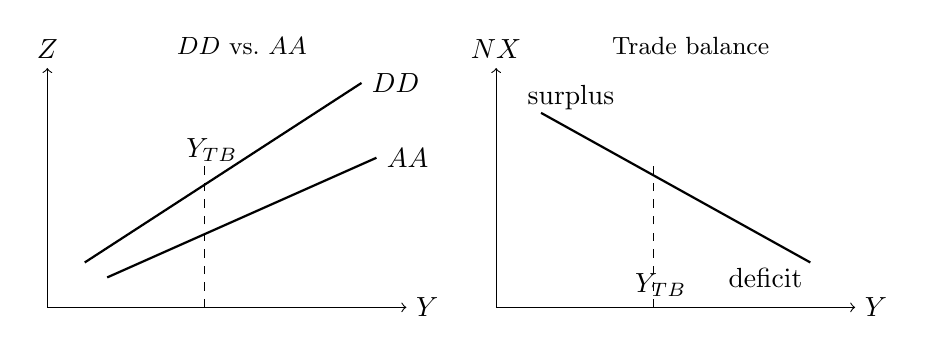
\begin{tikzpicture}[scale=0.95]
    \begin{scope}
      \node at (2.6,3.5) {\small $DD$ vs.\ $AA$};
      \draw[->] (0,0) -- (4.8,0) node[right] {$Y$};
      \draw[->] (0,0) -- (0,3.2) node[above] {$Z$};
      \draw[thick] (0.5,0.6) -- (4.2,3) node[right] {$DD$};
      \draw[thick] (0.8,0.4) -- (4.4,2.0) node[right] {$AA$};
      \draw[dashed] (2.1,0) -- (2.1,1.9);
      \node at (2.2,2.1) {$Y_{TB}$};
    \end{scope}
    \begin{scope}[xshift=6.0cm]
      \node at (2.6,3.5) {\small Trade balance};
      \draw[->] (0,0) -- (4.8,0) node[right] {$Y$};
      \draw[->] (0,0) -- (0,3.2) node[above] {$NX$};
      \draw[thick] (0.6,2.6) -- (4.2,0.6);
      \draw[dashed] (2.1,0) -- (2.1,1.9);
      \node at (2.2,0.3) {$Y_{TB}$};
      \node at (1.0,2.8) {surplus};
      \node at (3.6,0.4) {deficit};
    \end{scope}
  \end{tikzpicture}
  \caption{$DD$ vs.\ $AA$ and the corresponding trade-balance diagram, matching the handwritten sketches.}
\end{figure}

\subsection*{17-2 Equilibrium Output \& Trade Balance}
$Y=Z$ gives goods-market equilibrium; it need not align with $Y_{TB}$.

\subsection*{17-3 Increased Domestic Demand}
\begin{itemize}
  \item Assuming $Y^\ast = Y_{TB}$, higher $G$ shifts $ZZ$ up but creates a trade deficit.
  \item Multiplier smaller than in closed economy since $ZZ$ is flatter than $DD$.
\end{itemize}

\subsection*{17-4 Increases in Foreign Demand}
$\uparrow Y^\ast$ shifts $ZZ$ upward, improving the current account ($\Delta NX > 0$).

\subsection*{17-4b Depreciation, Trade Balance, Output}
Marshall--Lerner condition:
\[
  \frac{\Delta \varepsilon}{\varepsilon} + \frac{\Delta X}{X} - \frac{\Delta IM}{IM} > 0 \quad \Rightarrow \quad \Delta NX > 0.
\]
Depreciation shifts demand toward domestic goods $\Rightarrow \uparrow Y$, improved trade balance, but higher import prices reduce real income.

\subsection*{17-5 Dynamics: J-Curve}
After depreciation the trade balance can initially worsen because import values jump; over time, volumes adjust and NX improves.

\subsection*{17-6 Savings, Investment, Current Accounts}
\[
  CA = S + (T-G) - I.
\]
Usually $NX \approx CA - NI - NT$ with net income/transfers small.

\section*{CH.\ 18: Openness}

\subsection*{18-1 Goods Markets}
\begin{itemize}
  \item US has become more open; $NX$ usually negative.
  \item Real exchange rate $\varepsilon = E \cdot \frac{P^\ast}{P}$; appreciation $\Rightarrow$ domestic goods more expensive.
  \item Fixed exchange rates: revaluations ($\uparrow E$), devaluations ($\downarrow E$).
\end{itemize}

\subsection*{18-2 Financial Markets}
\begin{itemize}
  \item Need multilateral (trade-weighted) exchange rates when many partners are involved.
  \item Balance of payments:
    \begin{enumerate}
      \item Current account (above the line): trade balance, net income, net transfers.
      \item Capital account (below the line): net capital flows $\Rightarrow$ foreign holdings of domestic assets minus domestic holdings of foreign assets.
    \end{enumerate}
  \item Statistical discrepancy $=$ Current Account $-$ Capital Account.
  \item GNP $=$ GDP $+$ net income ($NI$, usually small).
  \item Openness of financial markets allows large FX volumes ($> \$4$T/day) and financing of trade deficits/surpluses.
\end{itemize}

\subsection*{Choice Between Domestic \& Foreign Assets}
Uncovered interest parity:
\[
  (1+i_t) = (1+i_t^\ast)\frac{E_t^e}{E_t} \quad \Rightarrow \quad i_t \approx i_t^\ast - \frac{E_{t+1}^e - E_t}{E_t}.
\]
Arbitrage equates expected returns unless governments tolerate large movements in $E$.

\section*{CH.\ 20: Output, Interest, Exchange Rate (Mundell--Fleming)}

\subsection*{20-1 Goods Market}
\[
  Y = C(Y-T) + I(Y,i) + G + NX(Y,Y^\ast,E),
\]
with $P$ (and $P^\ast$) given in the short run so $\pi_t^e = 0$ and $r_t = i_t$.

\subsection*{20-2 Financial Markets}
Money demand $\frac{M}{P} = Y \cdot L(i)$. Money vs.\ bonds: no difference (perfect substitutability). UIP links $i$ and $E$ via $(1 + i_t) = (1 + i_t^\ast)\frac{E_t^e}{E_t}$.

\subsection*{20-3 Goods+Financial Markets Together}
IS--LM in an open economy plus the interest parity (IP) relation. Fiscal policy affects both $Y$ and $E$; monetary policy affects $E$ via UIP.

\subsection*{20-4 Fiscal Policy in Open Economy}
Fiscal expansion: IS shifts right, raising $Y$, $i$, and appreciating the currency ($E$ falls), which worsens NX.

\subsection*{20-5 Fixed Exchange Rates}
\begin{itemize}
  \item \textbf{Peg:} currency is attached to another at fixed $E$.
  \item \textbf{Crawling peg:} predetermined rate of depreciation/appreciation.
  \item \textbf{EMS example:} exchange rates maintained within a narrow band around central parity; 1992 crisis precipitated the move toward the euro.
  \item With $E_t = E_{t+1}^e = \bar{E}$, UIP implies $i_t = i_t^\ast$. Thus $\frac{M}{P} = Y \cdot L(i^\ast)$ and the central bank cannot run an independent monetary policy; fiscal policy becomes the main stabilization tool.
\end{itemize}

\section*{CH.\ 21: Exchange Rate Regimes}

\subsection*{21-1 Medium Run with Fixed Rates}
AD depends on $\frac{E P^\ast}{P}$; if $P$ rises, the real exchange rate appreciates, shifting demand away from domestic goods until AS adjusts and $Y$ returns to $Y_n$.

\subsection*{21-2 Exchange Rate Crises \& Case for Devaluation}
\begin{itemize}
  \item Devaluation (lower $E$) quickly shifts AD outward and lowers the real wage, speeding the return to $Y_n$, but the improvement in $NX$ arrives with a lag (J-curve).
  \item Under floating rates $E$ adjusts freely; under fixed rates, expected devaluation forces $i$ higher:
  \[
    i_t = i_t^\ast - \frac{E_{t+1}^e - E_t}{E_t}.
  \]
  \item If markets assign probability $p$ to devaluation,
  \[
    i_t = i_t^\ast - \left[p\frac{E_{t+1}^d - E_t}{E_t} + (1-p)\frac{E_{t+1}^e - E_t}{E_t}\right].
  \]
  \item Governments can try to reassure markets (promise no devaluation), raise $i$, or eventually adjust the parity.
\end{itemize}

\subsection*{21-3 Flexible Exchange-Rate Movements}
\[
  E_t = \frac{1+i_t}{1+i_t^\ast} E_{t+1}^e
  \quad \Rightarrow \quad
  E_t = \prod_{\tau=0}^{n-1} \frac{1+i_{t+\tau}}{1+i^\ast_{t+\tau}} \, E_{t+n}^e.
\]
Hence $E_t$ moves one-for-one with expected future rates; long-run target (e.g., CA balance) anchors expectations but short-run $E_t$ can be volatile.

\section*{Fiscal Policy Appendix (CH.\ 23)}

\subsection*{23-2 Government Budget Constraint}
\[
  D_t = r B_{t-1} + G_t - T_t, \qquad \Delta B_t = D_t, \qquad B_t = (1+r)B_{t-1} + (G_t - T_t).
\]
Example: tax cut today ($B_1 = 1$) requires future primary surpluses to repay $1+r$.

\subsection*{Debt Stabilization}
\[
  \frac{\Delta B_t}{Y_t} = (r - g_Y)\frac{B_{t-1}}{Y_{t-1}} + \frac{G_t - T_t}{Y_t}.
\]
To stabilize debt, set $D_t = 0$; to reduce it, require primary surplus when $(r-g_Y) > 0$.

\subsection*{Ricardian Equivalence}
Under strong assumptions (infinitely lived altruistic families, perfect capital markets, fixed debt path) the timing of taxes does not affect demand: $G$ financed via debt or taxes has same effect on $Y$.

\subsection*{Deficits, Stabilization, Wars}
\begin{itemize}
  \item Cyclical-adjusted deficit is the benchmark when $Y = Y_n$.
  \item Wars lead to large deficits; tax smoothing suggests running deficits when spending needs are high and surpluses otherwise.
\end{itemize}

\subsection*{Dangers of High Debt}
\begin{itemize}
  \item Goal: stabilize and eventually reduce $B_t/Y_t$.
  \item Default: creditors take a haircut, with severe domestic and external implications.
  \item Money finance under fiscal dominance: central bank purchases government bonds via money creation ($\Delta H$).
  \item Seignorage revenue:
  \[
    \frac{\Delta H}{P} = \frac{\Delta H}{H} \cdot \frac{H}{P} = g(H) \cdot \frac{H}{P}.
  \]
  Financing a deficit equal to $x\%$ of GDP via seignorage requires $g(H) = x\%$; large $g(H)$ risks high inflation.
\end{itemize}

\section*{Note on Blank Pages}
Scans 6, 10, 14, 28, 32, 48, and 60 contained no legible handwritten content (likely blank backs of sheets); they are intentionally omitted.

\end{document}
